\documentclass{scrartcl}

\usepackage[utf8x]{inputenc}
\usepackage{array}
\usepackage{tabularx}
\usepackage{multirow}
\usepackage{graphicx}
\usepackage{booktabs}
\usepackage{caption}
\usepackage{subcaption}
\usepackage{titling}
\usepackage{xcolor}
\usepackage{amsmath}

\usepackage{amsfonts}
\usepackage{multicol}
\usepackage{wrapfig}

\usepackage[a4paper, margin=.9in]{geometry}
\usepackage{tikz}

\usepackage{enumitem}
\usepackage{amssymb}     % provides \blacktriangleright
\usetikzlibrary{shapes,decorations,arrows,calc,arrows.meta,fit,positioning}
\tikzset{
    -Latex,auto,node distance =1 cm and 1 cm,semithick,
    state/.style ={ellipse, draw, minimum width = 0.7 cm},
    point/.style = {circle, draw, inner sep=0.04cm,fill,node contents={}},
    bidirected/.style={Latex-Latex,dashed},
    el/.style = {inner sep=2pt, align=left, sloped}
}

\setlength{\droptitle}{-7.5em}

\title{Causal Inference for Policy Evaluation\\
\Large{Final Assignment}}
\author{Marco Gortan, Felix Schulz, Benjamin Weggelaar}
\date{\today}

\newcommand{\marco}[1]{\textcolor{red}{#1}}
\newcommand{\felix}[1]{\textcolor{cyan}{#1}}
\newcommand{\benji}[1]{\textcolor{green}{#1}}

\begin{document}

\maketitle



\subsection*{Difference-in-differences (DiD)}
% You want to exploit the introduction of the program to estimate its effects based on DiD. As outcome variables you want to use unemployment duration and the probability of being employed 12 months after entering unemployment

\paragraph*{1.}
% What would be the treatment group, and what would be the control group? Explain. [4
% points]
The treatment group is composed of those who participated in the training program during their unemployment spell in 2015, while the control group is composed of those who did not participate. The training program was introduced in 2013; therefore, we consider the pre-period as the unemployment spell in 2011. 

\paragraph*{2.}
% Generate the two outcome variables of interest and provide descriptive statistics for all four
% relevant groups (treated pre/post, controls pre/post). Discuss the results. [4 points]
Figure \ref{fig:combined} visually shows the outcome variables for the four relevant groups.

\begin{figure}[h!]
  \centering
  %–––––––––––––––––––––––––––––––––––––––––––––––––––––––––––––––––––––––––
  \begin{subfigure}[t]{0.48\textwidth}
    \centering
    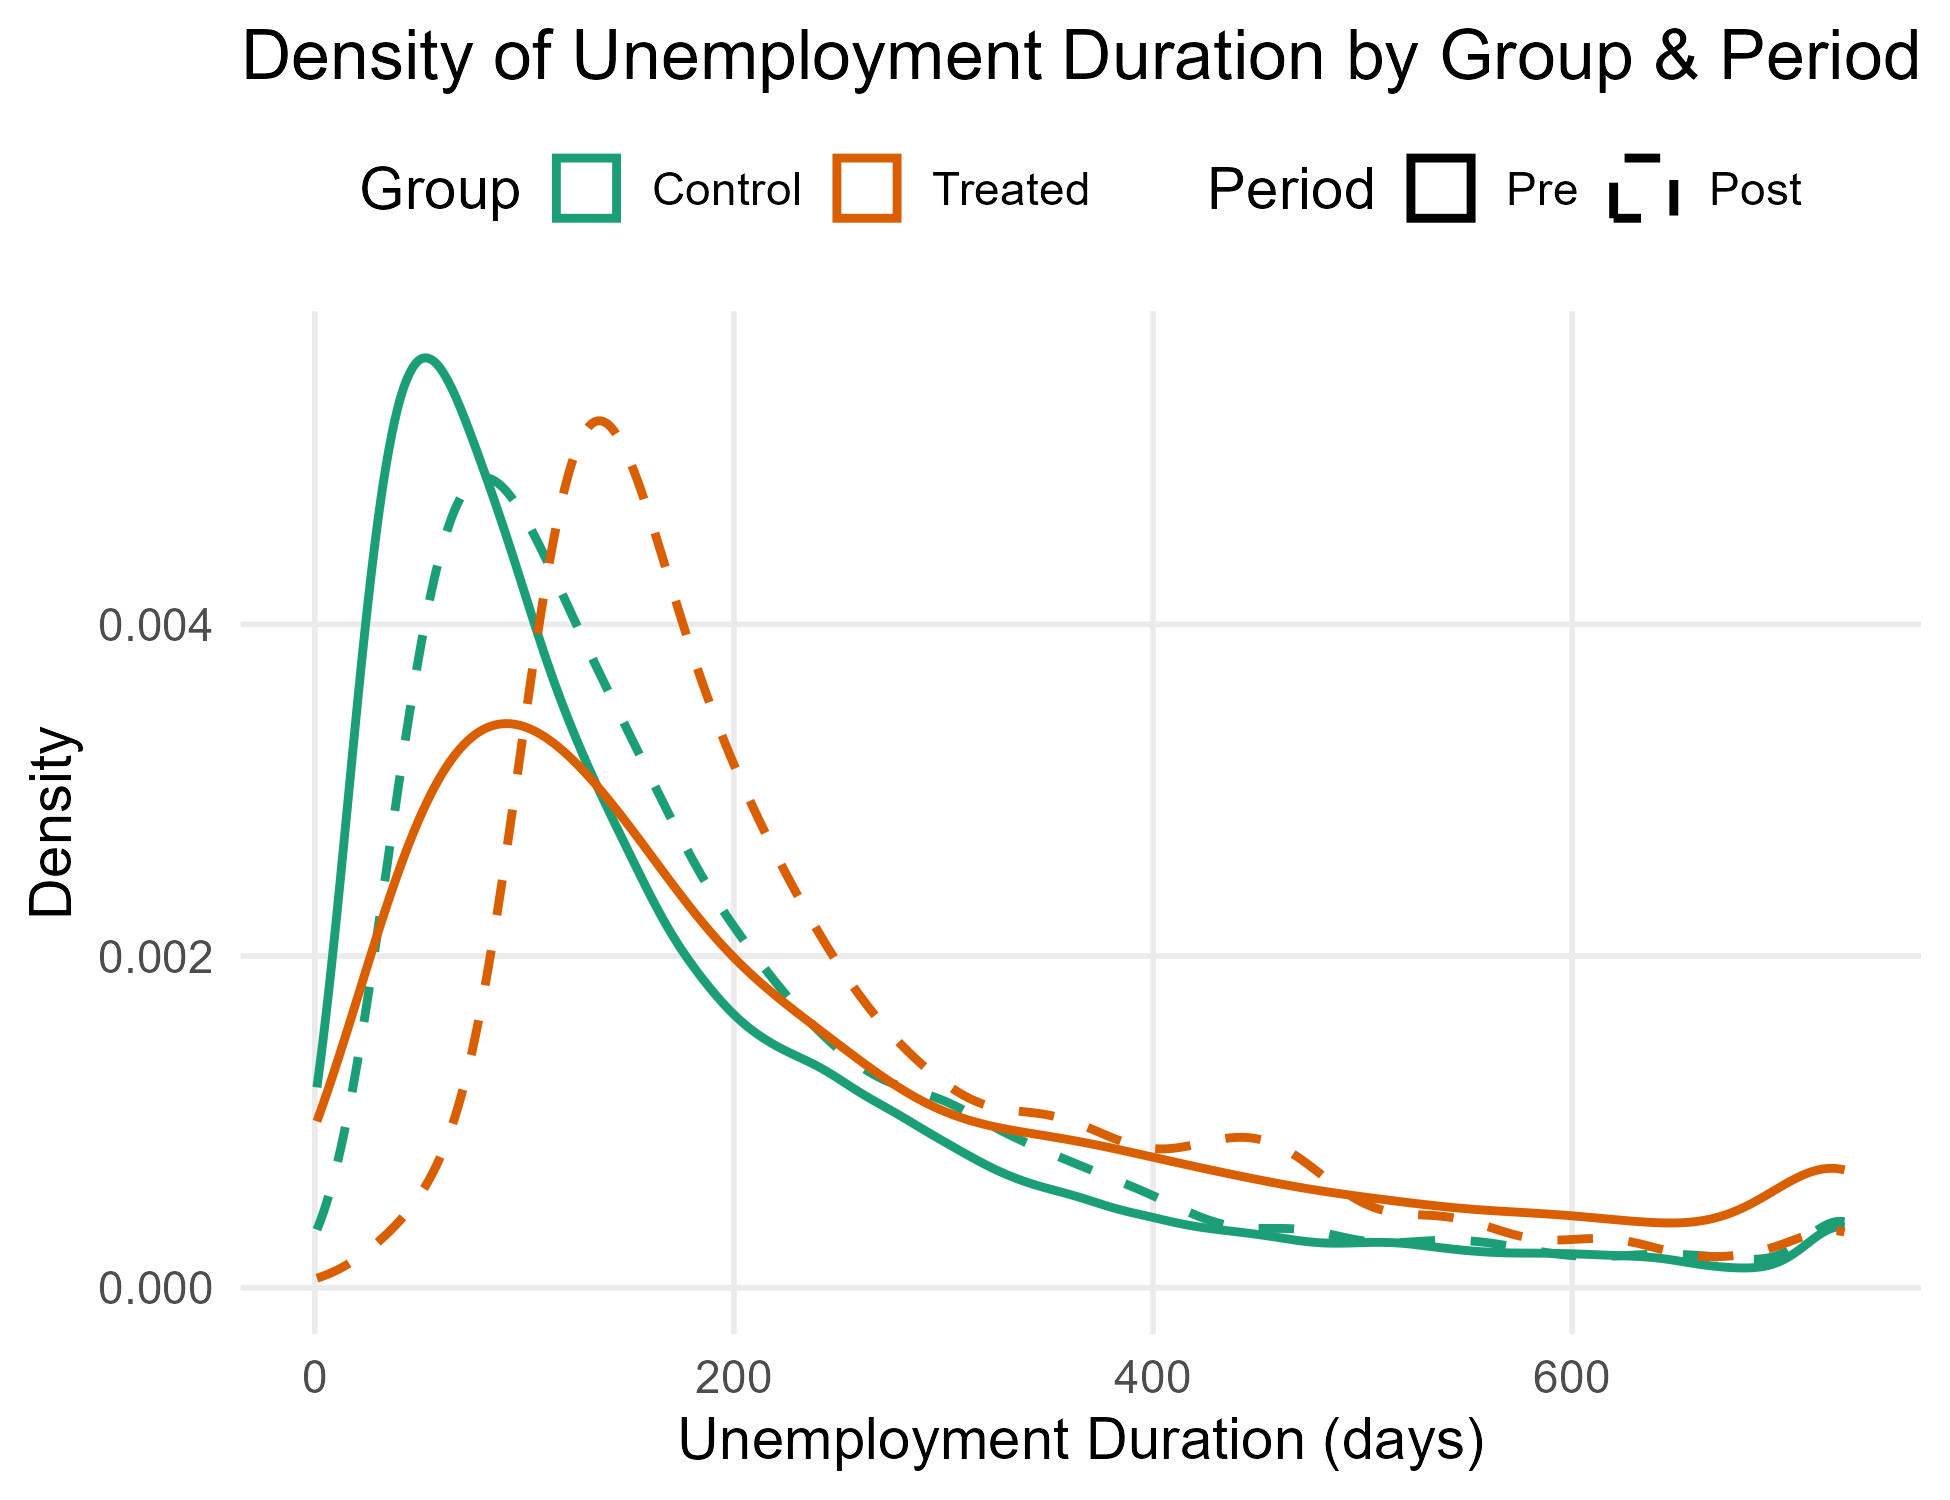
\includegraphics[width=\linewidth]{output/figures/final_unemployment_duration_density.jpg}
    \caption{Density of unemployment duration by group \& period}
    \label{fig:density}
  \end{subfigure}
  \hfill
  \begin{subfigure}[t]{0.48\textwidth}
    \centering
    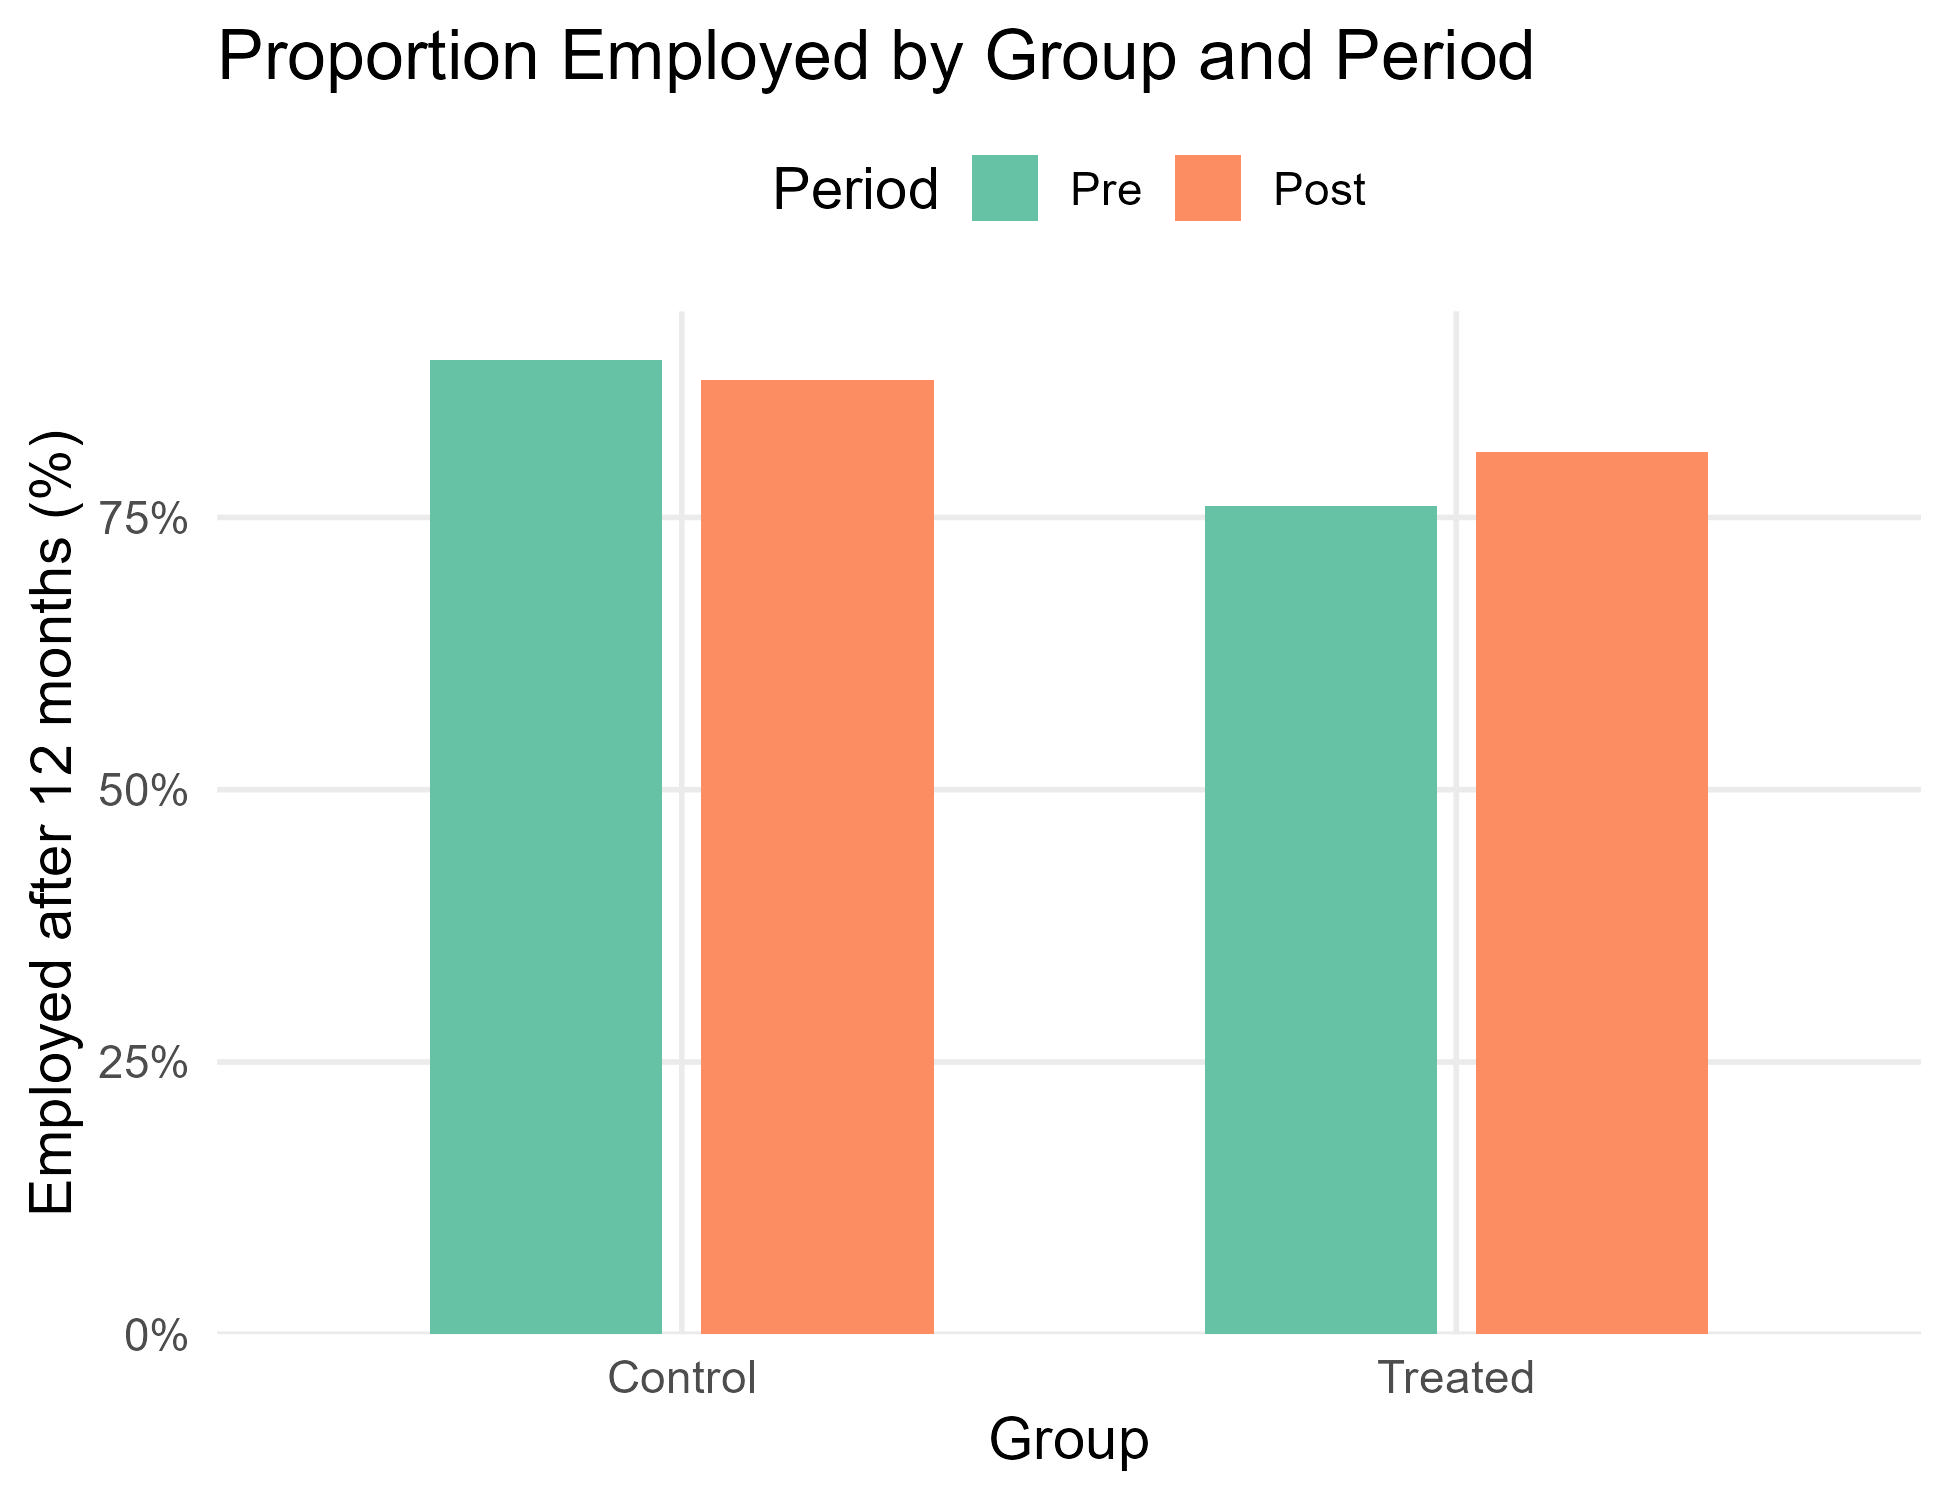
\includegraphics[width=\linewidth]{output/figures/final_employment12m.jpg}
    \caption{Proportion employed after 12 months by group \& period}
    \label{fig:employment}
  \end{subfigure}
  %–––––––––––––––––––––––––––––––––––––––––––––––––––––––––––––––––––––––––
  \caption{Visual representation of the outcome variables for the four relevant groups.}
  \label{fig:combined}
\end{figure}



\paragraph*{3.}
% Compare mean observed characteristics for all four relevant groups (treated pre/post, controls
% pre/post). Discuss the results. [6 points]

Table \ref{tab:tab:final_mean_char} shows the mean observed characteristics for all four relevant groups. We note that treated people:

\begin{itemize}[label=$\blacktriangleright$]
    \item \textbf{Are older}. This is expected given how the policy has been implemented; \
    \item \textbf{Are prevalently women}; \
    \item \textbf{Have higher insured earnings.} This might reglect that they are older compared to non-treated; \
    \item \textbf{Had higher part-time rates}. ;\
    \item \textbf{Receive more children subsidies.} Again, this might reflect that they are older than non-treated; \
    \item \textbf{Have worked a similar number of months preceding unemployment}. 
\end{itemize}

\begin{table}[!h]
\centering
\caption{\label{tab:tab:final_mean_char}Descriptive Statistics by Treatment Group and Period}
\centering
\resizebox{\ifdim\width>\linewidth\linewidth\else\width\fi}{!}{
\begin{tabular}[t]{rrrrrrrrrr}
\toprule
\multicolumn{2}{c}{ } & \multicolumn{3}{c}{Demographics} & \multicolumn{2}{c}{Economic} & \multicolumn{3}{c}{Other} \\
\cmidrule(l{3pt}r{3pt}){3-5} \cmidrule(l{3pt}r{3pt}){6-7} \cmidrule(l{3pt}r{3pt}){8-10}
Treatment & Post & N & Age (yrs) & Female (\%) & Married (\%) & Earnings & Act. rate (\%) & Child sub. (\%) & Contr. 2y (m)\\
\midrule
0 & 0 & 8080 & 29.5 & 56.1 & 21.6 & 4482.8 & 93.1 & 6.6 & 10.8\\
0 & 1 & 8292 & 32.8 & 55.9 & 23.5 & 4404.0 & 88.7 & 11.0 & 10.0\\
1 & 0 & 3692 & 49.1 & 59.1 & 49.2 & 5285.6 & 86.5 & 9.0 & 11.8\\
1 & 1 & 3898 & 53.0 & 57.7 & 47.5 & 5200.5 & 82.9 & 13.6 & 10.9\\
\bottomrule
\end{tabular}}
\end{table}


\paragraph*{4.}
% Which assumptions do you need to identify the effect of interest based on DiD in this setup?
% [5 points]

We need:

\begin{itemize}[label=$\blacktriangleright$]
    \item \textbf{Stable unit treatment value assumption (SUTVA).} Each unit’s potential outcome under a given treatment depends only on its own treatment assignment, not on the treatments received by any other units;\
    \item \textbf{No anticipation assumption (NA)}. \
    \item \textbf{Common trend assumption (CT).} Treated and controls are subject to the same time trend in the absence of treatment. \
    \item \textbf{Exogeneity assumption (EX)}. Covariates are unaffected by treatment.\ 
    \item \textbf{Common support (CS)}. Comparable observations in all groups.
\end{itemize}

\paragraph*{5.}
% Plot average outcomes for treatment and control group for each month in the observation
% period. Discuss the results. [6 points]

Figure \ref{fig:combined_overtime} shows the evolution of the outcome variables over time in the observation period. We notice that the employment rate for the treated is virtually zero in the first three months after they enter unemployment. This is likely because the program lasts 3 months, during which their ability to look for a job is arguably low. The dashed line shows the values of the outcomes starting from the beginning of the program instead of from the beginning of the unemployment spell. Employment rates and unemployment duration mechanically appear better and more similar to the non-treated group.

\begin{figure}[h!]
  \centering
  %–––––––––––––––––––––––––––––––––––––––––––––––––––––––––––––––––––––––––
  \begin{subfigure}[t]{0.48\textwidth}
    \centering
    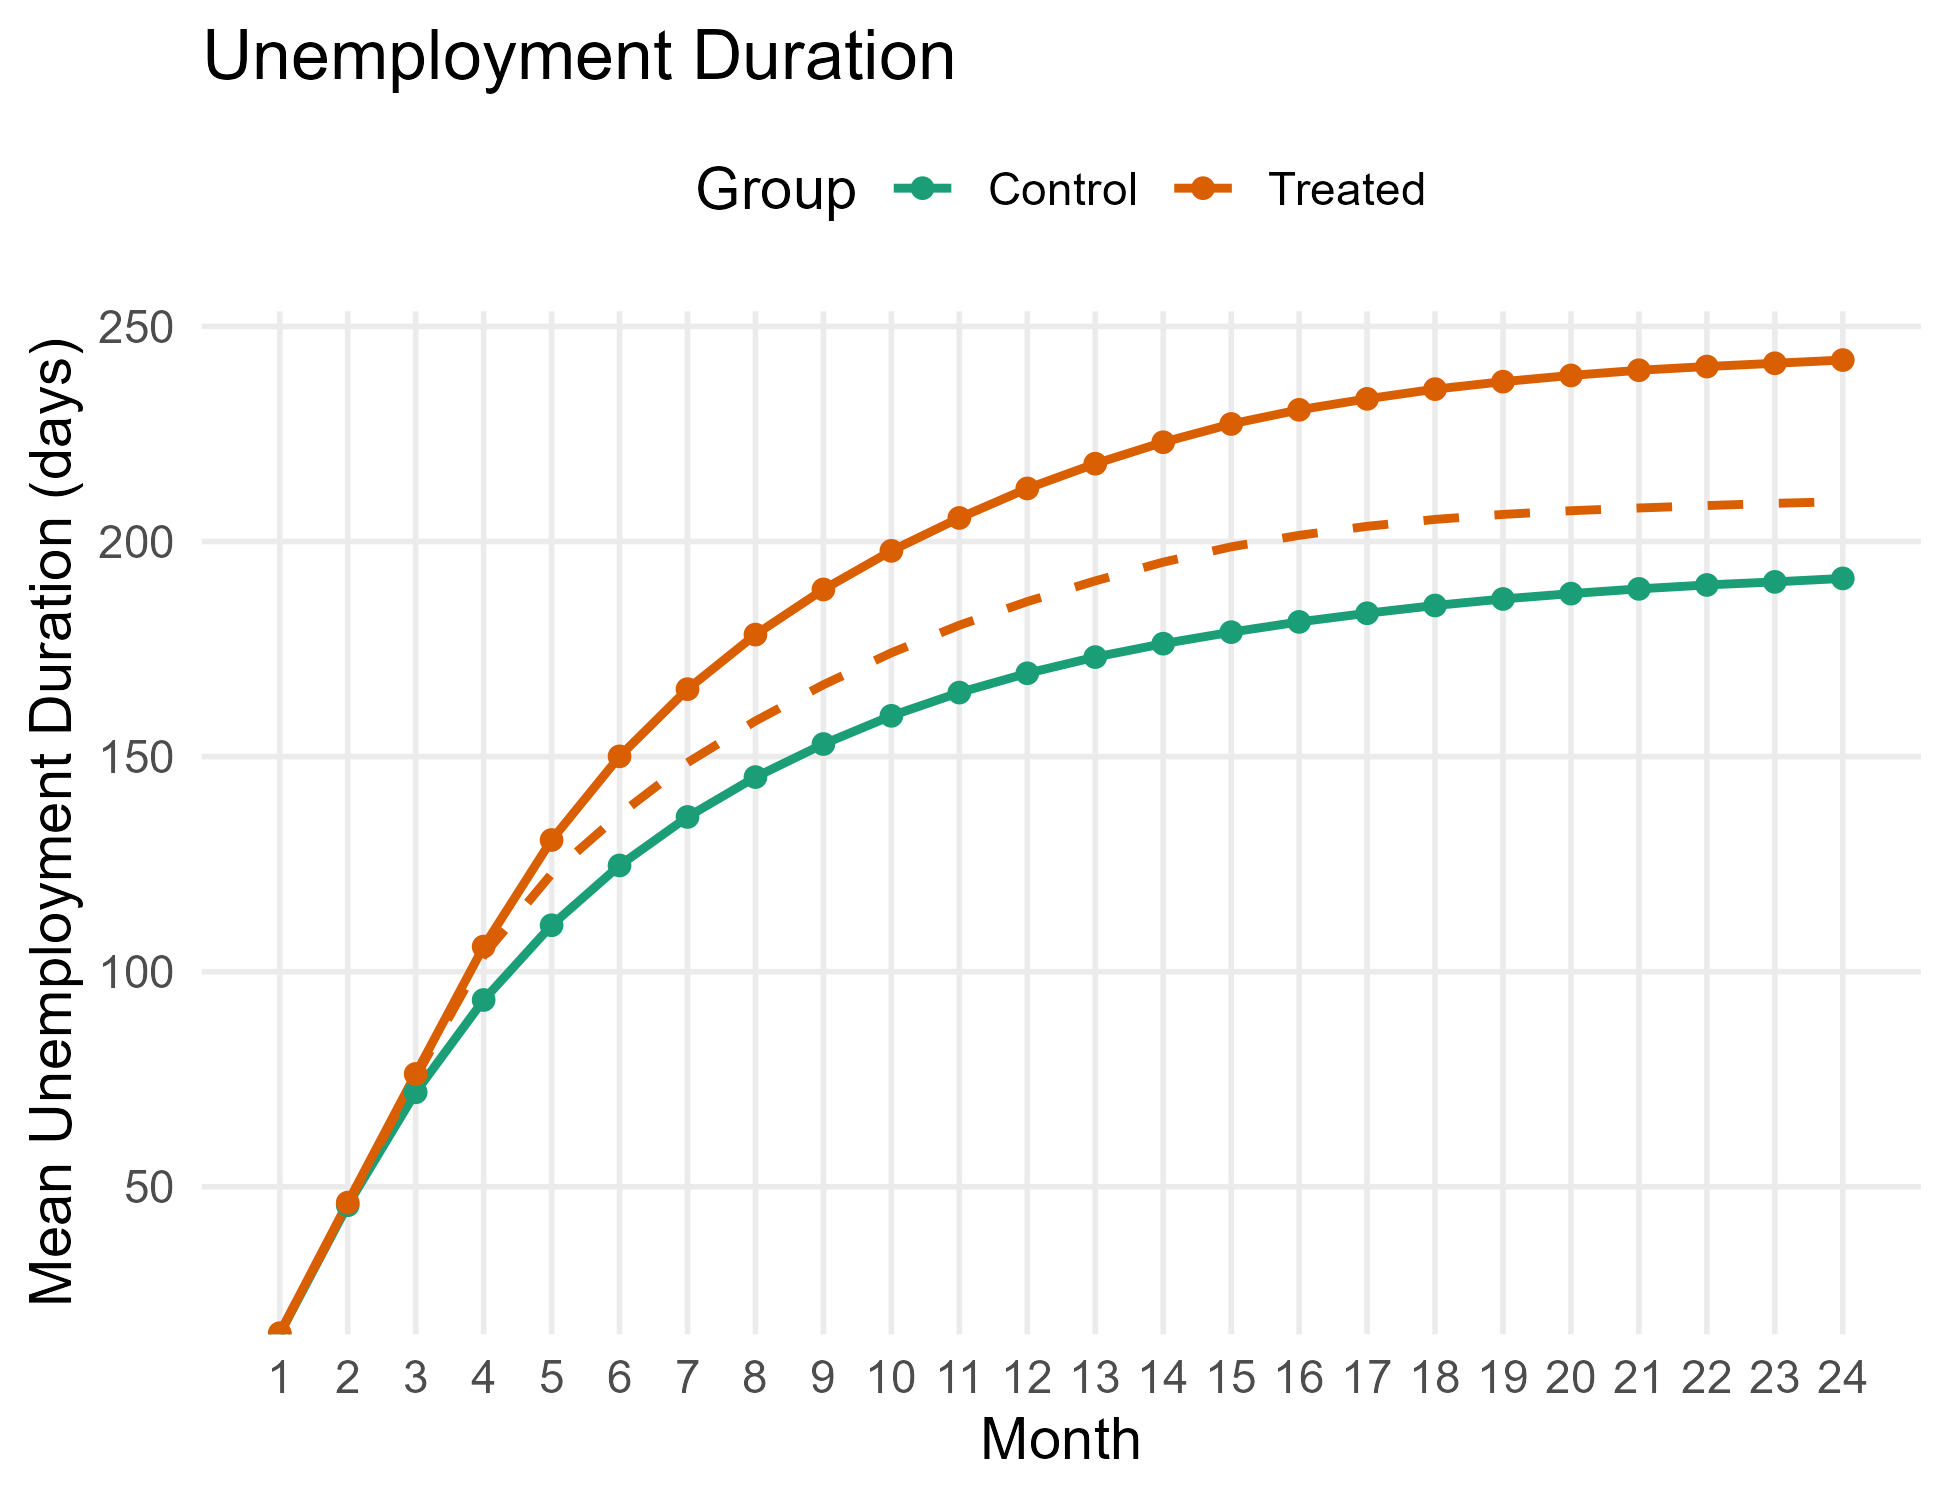
\includegraphics[width=\linewidth]{output/figures/final_unemployment_duration_over_time.jpg}
    \caption{}
    \label{fig:duration_overtime}
  \end{subfigure}
  \hfill
  \begin{subfigure}[t]{0.48\textwidth}
    \centering
    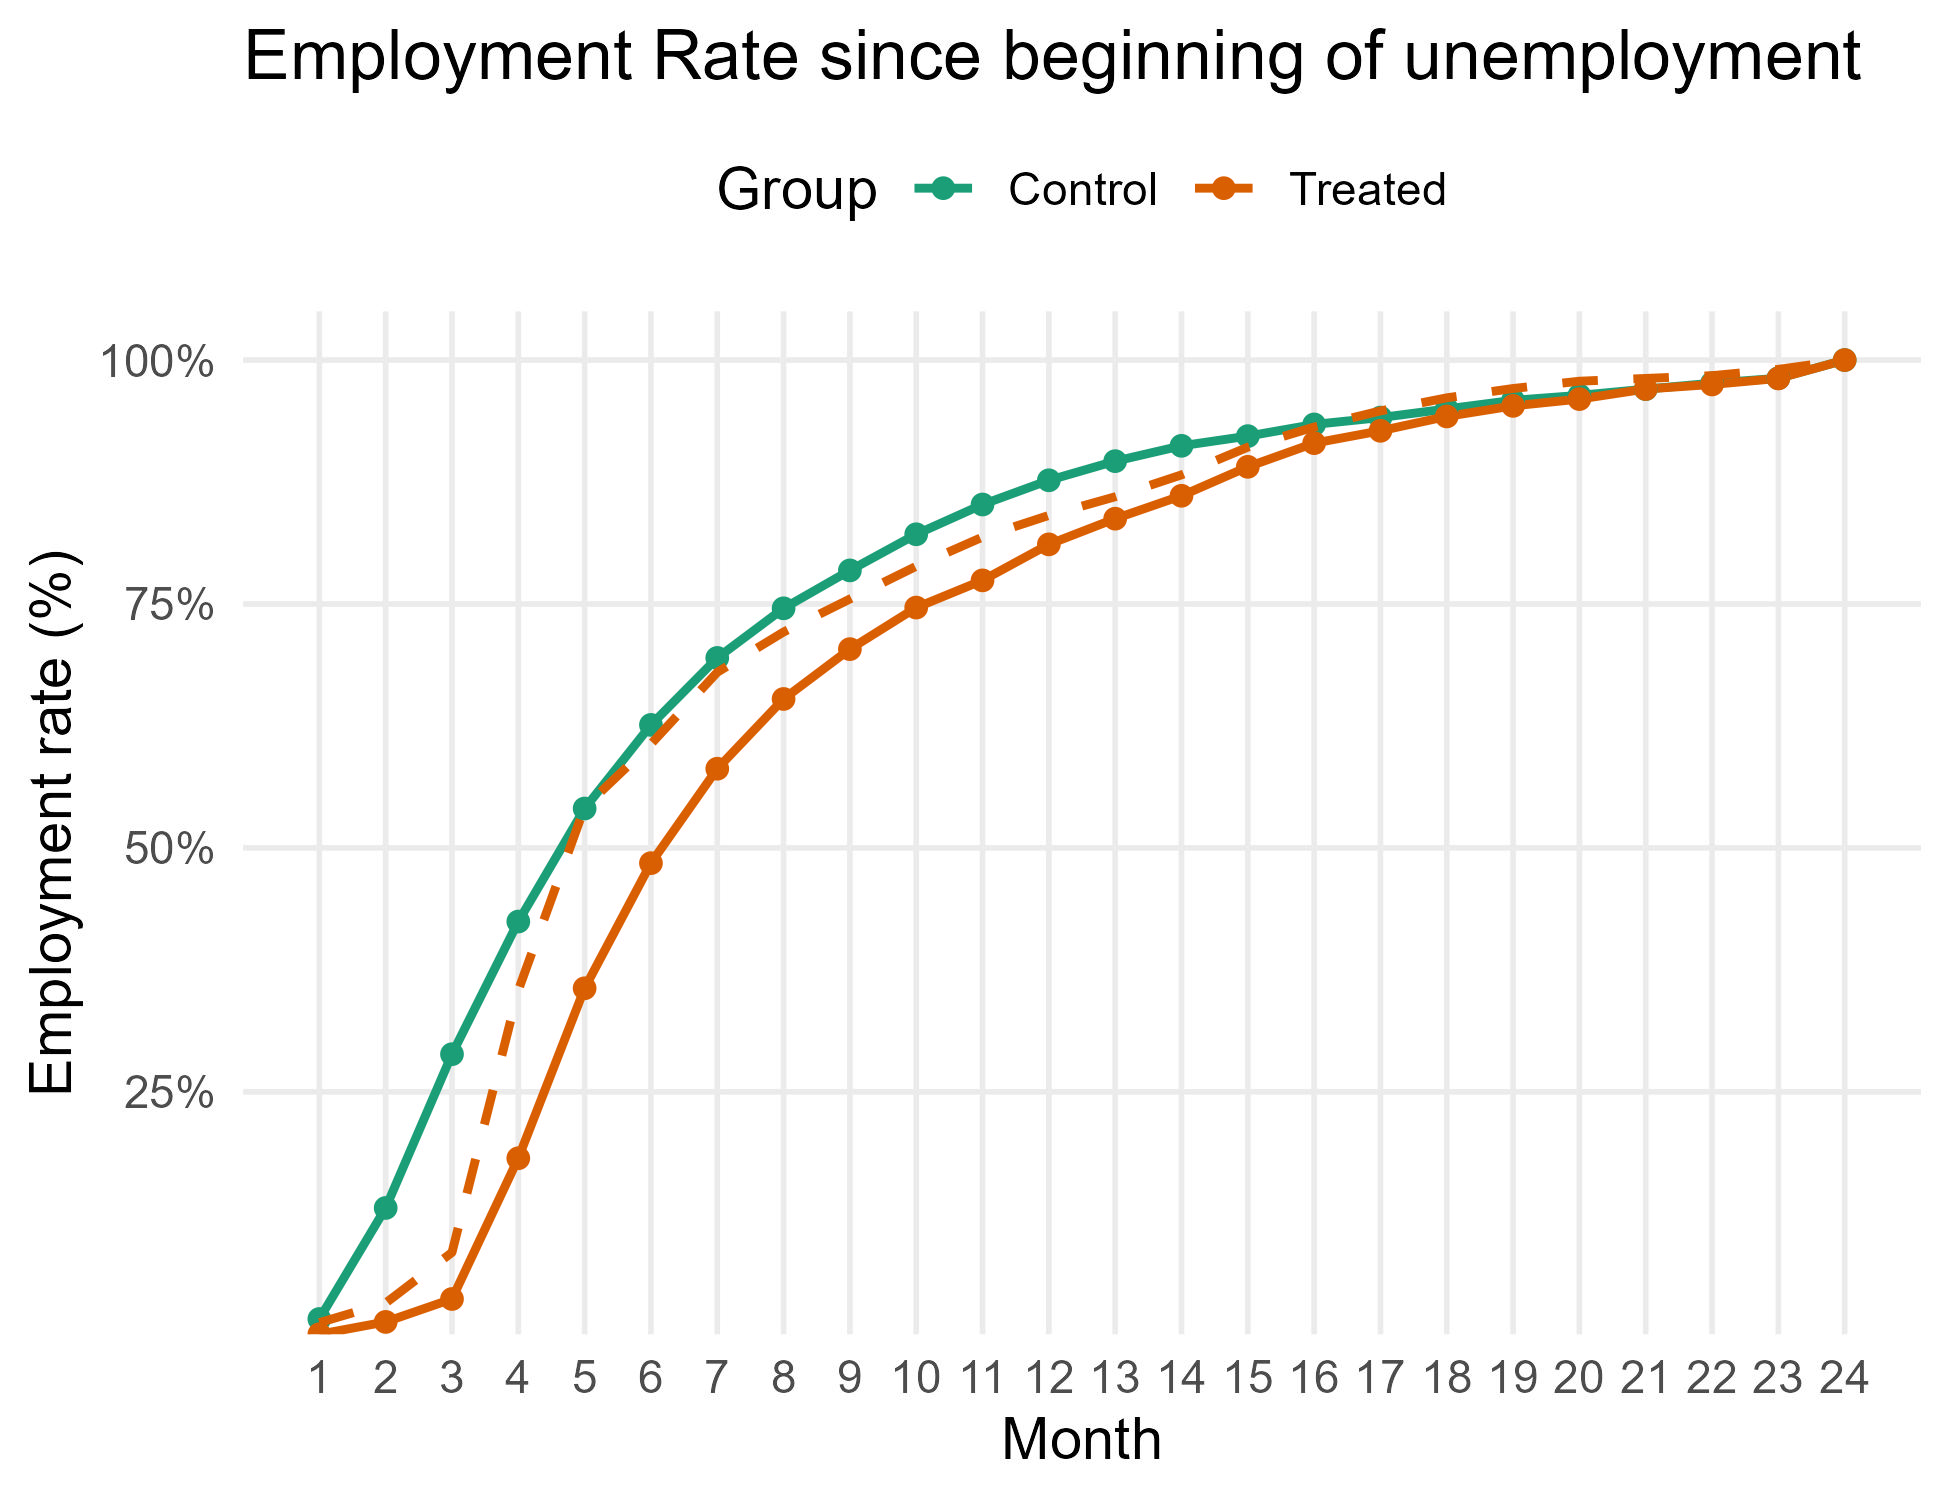
\includegraphics[width=\linewidth]{output/figures/final_employment_rate_over_time.jpg}
    \caption{Probability of being employed after x months}
    \label{fig:employment_overtime}
  \end{subfigure}
  %–––––––––––––––––––––––––––––––––––––––––––––––––––––––––––––––––––––––––
  \caption{Visual representation of the outcome variables over time in the observation period.}
  \label{fig:combined_overtime}
\end{figure}


\paragraph*{6.}
% Discuss the validity of the identifying assumptions in this specific case. Provide and discuss supporting evidence if possible, incl. event study estimates. [8 points]

\begin{itemize}[label=$\blacktriangleright$]
    \item \textbf{Stable unit treatment value assumption (SUTVA)}. SUTVA is not respected in case not-participating people are affected by those who join the program. It's possible that competition effects arise because many people apply for the same position and those who participated in the program win at the expense of others. However, it's also true that such programs might help reduce the mismatch between the skills looked for by employers and the skills of the employees. In that case, SUTVA is respected;\

    \item \textbf{No anticipation assumption (NA)}. According to the text, `\textit{Prior discussions about this policy change have remained confidential, so that neither caseworkers nor the unemployed had knowledge about it before this date}. If that is true, then this assumption is respected. \

    \item \textbf{Common trend assumption (CT).} Sadly, we do not have a panel structure present in the data, not allowing us to compute an event study to observe pre-treatment trends. Figure~\ref{fig:age_hist} shows that takeup of treatment is near universal in the treatment group. We therefore believe that self-selection into treatment is minimal. While we believe re-entry into the labor market is likely harder the older an individual is, there is no reason to believe this has changed around the program introduction. Therefore we believe that we have a good case for the CT assumption to hold.\ 

    \item \textbf{Exogeneity assumption (EX)}. :\ 

    \item \textbf{Common support (CS)}. Treated and non-treated mainly differ in age. Therefore, people below 45 are for sure part of the non-treated cohort. Similarly, people older than 45 are very likely to be part of the treated (see Figure \ref{fig:age_hist}).
\end{itemize}

\begin{figure}
    \centering
    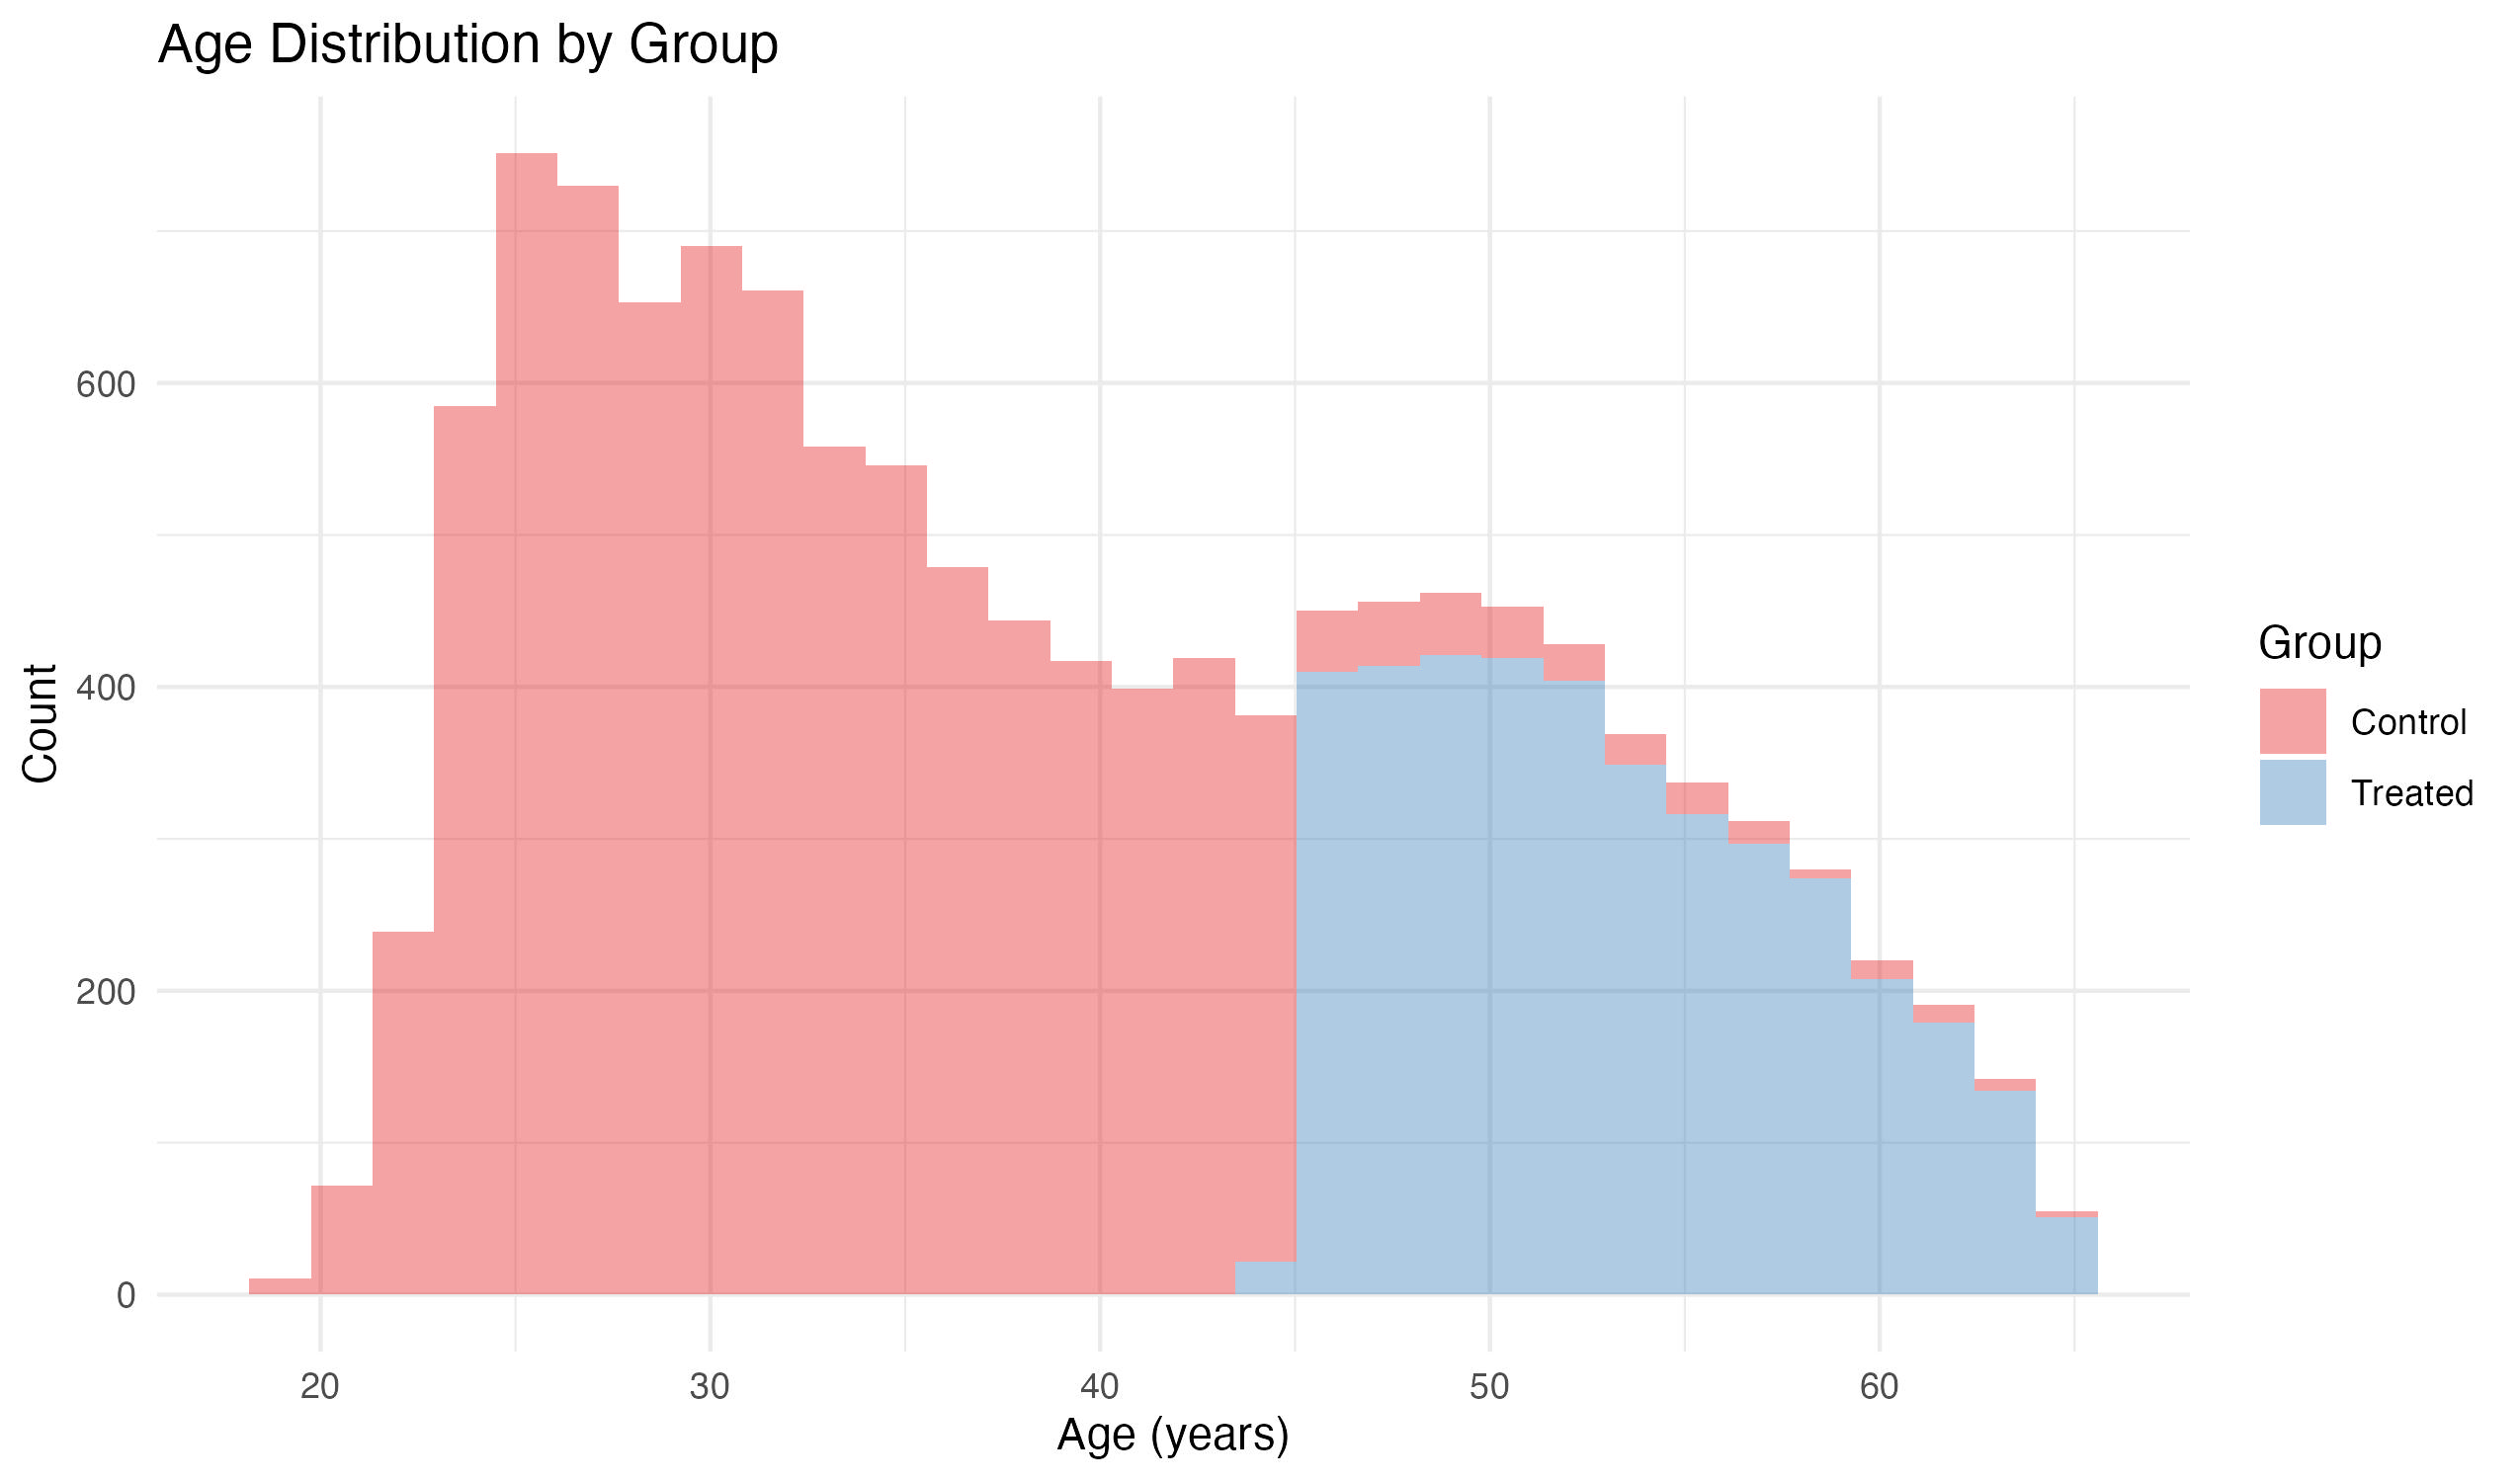
\includegraphics[width=0.75\linewidth]{output/figures/final_histogram_age.jpg}
    \caption{Age groups among treated and non-treated in the observation period.}
    \label{fig:age_hist}
\end{figure}

\paragraph*{7.}
% Implement the DiD using OLS. Describe in detail what you do and why. Discuss whether or
% not you need additional control variables and if so, why. Discuss the results. [8 points]

We estimate the model
$$
Y_{it} = \alpha + \beta_1 \text{Treat}_i + \beta_2 \text{Post}_t + \beta_3 (\text{Treat}_i \times \text{Post}_t) + \epsilon_{it}
$$
where \( Y_{it} \) is the outcome of interest for unit \( i \) at time \( t \), \( \text{Treat}_i \) is an indicator variable equal to 1 if the unit belongs to the treatment group, \( \text{Post}_t \) is an indicator equal to 1 for the post-treatment period, and the interaction term \( \text{Treat}_i \times \text{Post}_t \) captures the difference-in-differences (DiD) estimator \( \beta_3 \), which is our main coefficient of interest.

We estimate the model using Ordinary Least Squares (OLS). We believe that, for the reasons stated above, the common trends assumption holds unconditionally, meaning it does not depend on the inclusion of covariates. Nevertheless, because adding covariates can increase precision and help control for residual confounding, we also present results controlling for.


% Table created by stargazer v.5.2.3 by Marek Hlavac, Social Policy Institute. E-mail: marek.hlavac at gmail.com
% Date and time: Wed, Jul 02, 2025 - 17:51:03
\begin{table}[!htbp] \centering 
  \caption{OLS Results for Unemployment Duration} 
  \label{} 
\begin{tabular}{@{\extracolsep{5pt}}lcc} 
\\[-1.8ex]\hline 
\hline \\[-1.8ex] 
 & \multicolumn{2}{c}{\textit{Dependent variable:}} \\ 
\cline{2-3} 
\\[-1.8ex] & \multicolumn{2}{c}{Unemployment Duration (days)} \\ 
\\[-1.8ex] & (1) & (2)\\ 
\hline \\[-1.8ex] 
 Treated & 78.798$^{***}$ & 40.963$^{***}$ \\ 
  & ($-$2.963) & (19.965) \\ 
  & & \\ 
 Post & 27.363$^{***}$ & 21.677$^{***}$ \\ 
  & ($-$0.290) & (0.566) \\ 
  & & \\ 
 Treated * Post &  & 1.528$^{***}$ \\ 
  &  & ($-$1.429) \\ 
  & & \\ 
 sex &  & 5.419$^{*}$ \\ 
  &  & ($-$10.826) \\ 
  & & \\ 
 marits &  & 15.070$^{***}$ \\ 
  &  & ($-$0.012) \\ 
  & & \\ 
 insured\_earn &  & 0.001 \\ 
  &  & (0.001) \\ 
  & & \\ 
 lastj\_rate &  & $-$0.162$^{*}$ \\ 
  &  & ($-$0.939) \\ 
  & & \\ 
 child\_subsidies &  & 22.562$^{***}$ \\ 
  &  & ($-$1.286) \\ 
  & & \\ 
 contr\_2y &  & 1.573$^{***}$ \\ 
  &  & ($-$0.544) \\ 
  & & \\ 
 treat\_group:post & $-$28.033$^{***}$ & $-$28.263$^{***}$ \\ 
  & (0.290) & (1.683) \\ 
  & & \\ 
 Constant & 164.055$^{***}$ & 106.955$^{***}$ \\ 
  & (2.963) & (135.690) \\ 
  & & \\ 
\hline \\[-1.8ex] 
Observations & 23962 &  \\ 
R-squared & 0.038 &  \\ 
Observations & 23,855 & 23,855 \\ 
R$^{2}$ & 0.038 & 0.054 \\ 
Adjusted R$^{2}$ & 0.038 & 0.054 \\ 
\hline 
\hline \\[-1.8ex] 
\textit{Note:}  & \multicolumn{2}{r}{$^{*}$p$<$0.1; $^{**}$p$<$0.05; $^{***}$p$<$0.01} \\ 
\end{tabular} 
\end{table} 


\paragraph*{8.}
% Implement the DiD using a semi-parametric estimator based on the propensity score. Describe
% in detail what you do and why. Discuss the results and compare them to the OLS estimates.
% [10 points]
Problem of normal parametric diff-in-diff is that if (i) individual characteristics are associated with the outcome variable and (ii) characteristics are imbalanced over the groups, then it's likely that common trend assumption does not hold [this is some info I found on the PDF I uploaded in the GitHub]. Therefore, reweighting...

\paragraph*{9.}
% Discuss different ways of exploiting the panel structure of the data and implement one of them.
% Discuss to which extent the panel approach relaxes assumptions underlying the estimation
% approaches you used before. Describe in detail what you do and why. Discuss the results and
% compare them the other estimates. [10 points]

% Maybe do something staggered? 


\paragraph*{10.}
% Check for heterogeneous program effects with respect to observed characteristics for which
% you suspect different effects. Describe in detail what you do and why. Discuss the results. [5
% points]










\end{document}